\subsection{Helligkeitsverteilung}
\begin{table}[h!]
    \centering
    \begin{tabular}{ | l | c | c | c |}
        \hline
        Konfiguration & Beste & Unter 60 kB & Unter 28 kB \\\hline
        Ensemble-Methode & ExtraTrees & ExtraTrees & ExtraTrees \\\hline
        Maximalhöhe & 14 & 10 & 15 \\\hline
        Waldgröße & 10 & 6 & 1 \\\hline
        min\_samples\_leaf & 4 & 4 & 4 \\\hline
        Programmgröße in Bytes & 76628 & 33284 & 9364 \\\hline
        Genauigkeit Testmenge von Klisch & 74,0\% & 63,5\% & 67,7\% \\\hline
        Genauigkeit Gestentestmenge & 74,1\% & 79,2\% & 76,6\% \\\hline
        Genauigkeit Nullgestentestmenge & 69,0\% & 71,0\% & 67,0\% \\\hline
    \end{tabular}
    \caption{Beste Konfigurationen der Helligkeitsverteilung.}
    \label{tab:helligkeitsverteilung}
\end{table}
\begin{figure}[h!]
    \centering
    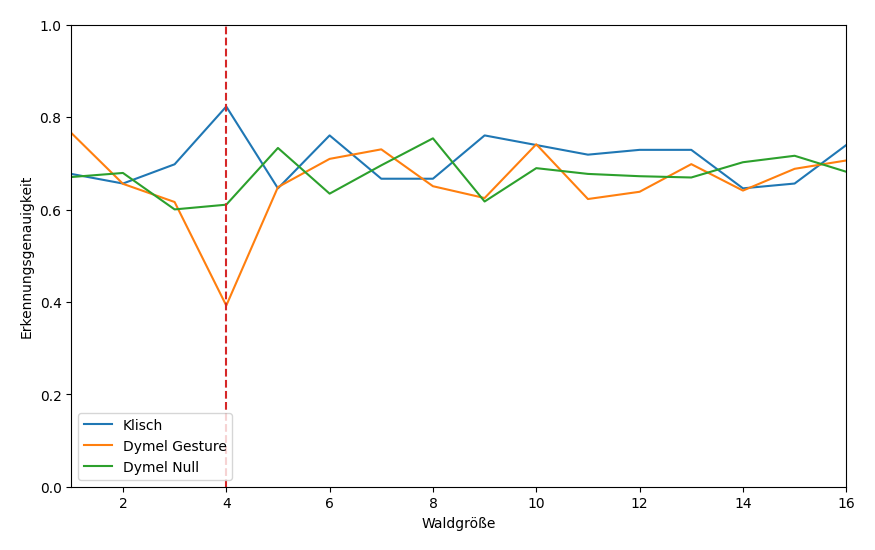
\includegraphics[width=\linewidth]{images/helligkeitsverteilung_acc_per_size.png}
    \caption{Die beste summierte Erkennungsgenauigkeit pro Waldgröße mit der Helligkeitsverteilung.}
    \label{fig:helligkeitsverteilung_per_forest_size}
\end{figure}
Die Featuremenge der Helligkeitsverteilung beinhaltet insgesamt 12 Features. Jeweils 6 Feature repräsentieren Zeitfenster der Minimalen Helligkeit und der Maximalen Helligkeit. Die Zeitfenster wurden
geometrisch zusammengefasst.
\newline
\newline
Die beste Konfiguration wurde mit der Ensemble-Methode \textit{ExtraTrees} gefunden (siehe Tabelle \ref{tab:helligkeitsverteilung}). Sie erzielt eine Erkennungsgenauigkeit von 74\% auf der Testmenge von Klisch
und ist damit 26\% schlechter als das neuronale Netzwerk von Giese \cite{gieseThesis}. Außerdem wird 74\% der Gestentestmenge und 69\% der Nullgestentestmenge korrekt klassifiziert.
\newline
\newline
Wird die beste Konfiguration mit der \textit{Unter 28 kB} vergleichen, nimmt die Gesamterkennungsgenauigkeit nur um 1,94\% ab bei einer Reduktion der Programmgröße von 87,8\%.
Ein ähnliches Verhalten ist auch in Abbildung \ref{fig:helligkeitsverteilung_per_forest_size} zu erkennen, indem die Gesamterkennungsgenauigkeit nur leicht mit der zunehmenden Waldgröße steigt.